\documentclass{article}
\usepackage[utf8]{inputenc}
\usepackage{caption}
\usepackage{graphicx}
\usepackage{listings}
\usepackage[framed,numbered,autolinebreaks,useliterate]{mcode}



\title{ENGN4528 Computer Vision Clab1 Report}
\author{Zhipeng Bao ~~ u6600985}
\date{March 2018}

\begin{document}

\maketitle

\section{Task 1: Basic Image I/O}
\subsection*{Step 1: Take three photos}
\subsection*{Step 2: Resize and restore the photos}
The three resized photos are in the attachments. 
\subsection*{Step 3: Basic operations on the image.}
\subsubsection*{3.1 \& 3.2 Resize image and show image}
This task is quite easy, the result and the codes are shown as follows:

\begin{figure}[htbp]
    \centering
    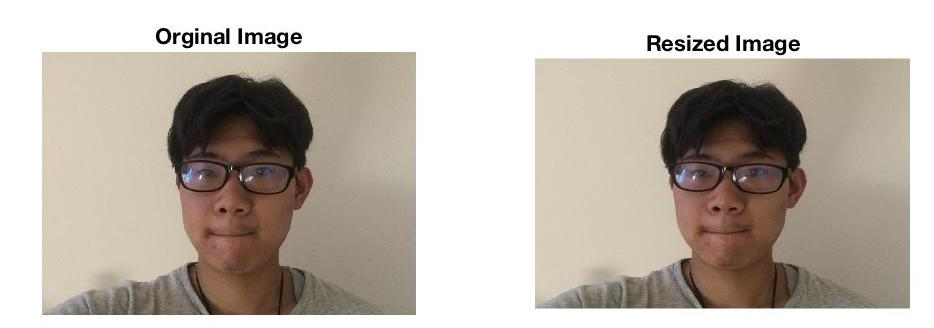
\includegraphics[scale = 0.3]{fig1.jpg}
    \caption{Face image: face\_01}
    \label{fig1}
\end{figure}

\begin{lstlisting}
    %3.1 e.g. select face_01
    image_name = 'face_01_u6600985.jpg';
    origin = imread(image_name);
    edit = imresize(origin, [512 768]);
    %3.2
    figure;
    subplot(1,2,1);
    imshow(origin);
    title('Orginal Image');
    subplot(1,2,2);
    imshow(edit);
    title('Resized Image');
\end{lstlisting}

\subsubsection*{3.3 Convert the image to RGB Channels}
Codes:
\begin{lstlisting}
    %3.3
    r = origin(:,:,1);
    g = origin(:,:,2);
    b = origin(:,:,3);
    figure;
    imshow(r);
    title('R channel grayscale image');
    figure;
    imshow(g);
    title('G channel grayscale image');
    figure;
    imshow(b);
    title('B channel grayscale image');
\end{lstlisting}
Result:
\begin{figure}[htbp]
    \centering
    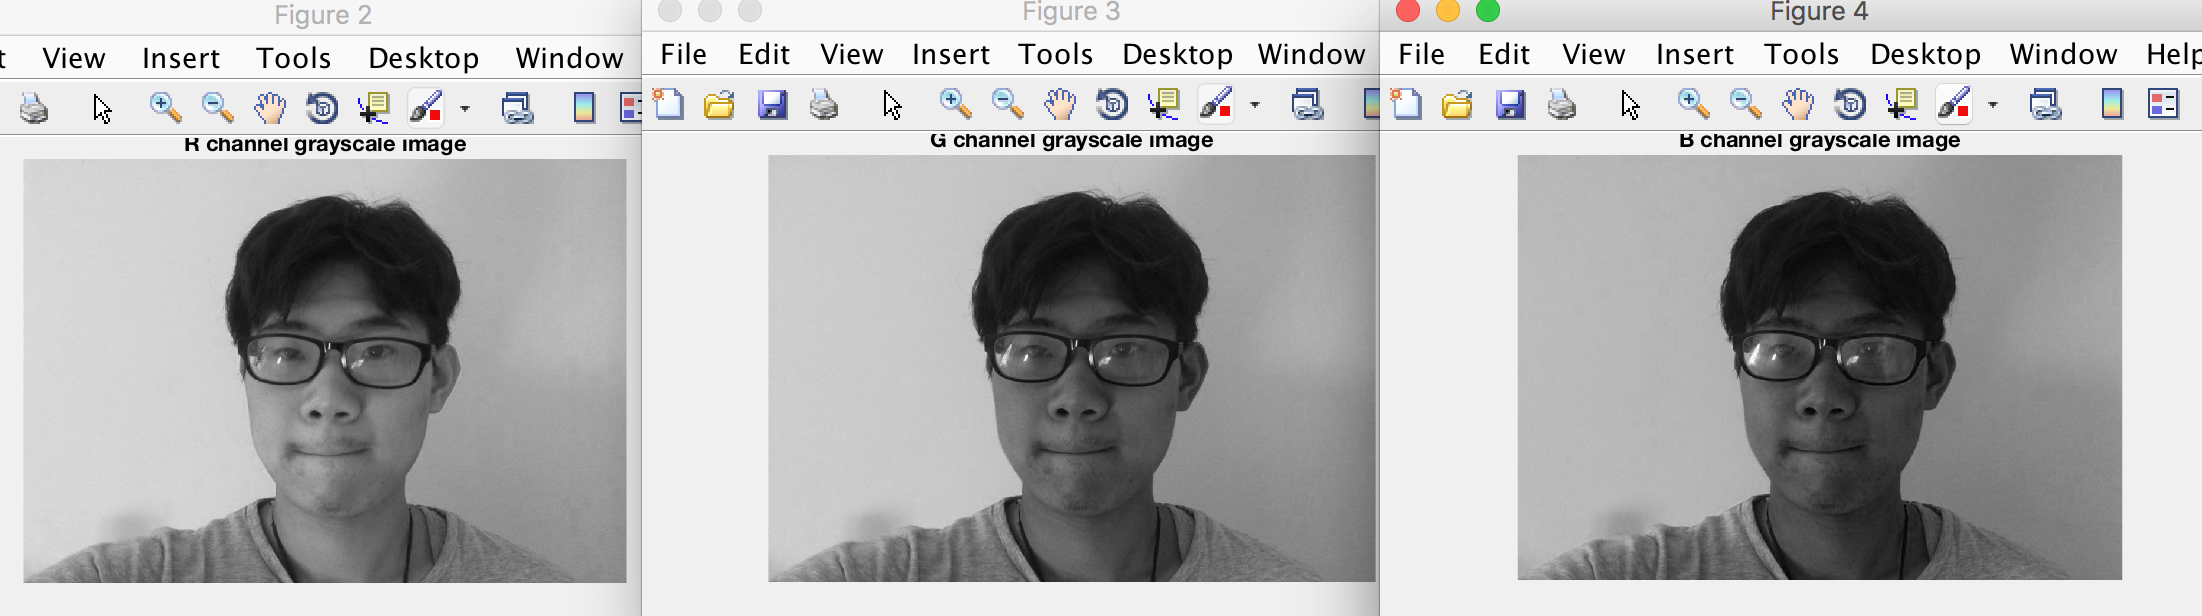
\includegraphics[scale = 0.3]{fig2.jpg}
    \caption{RGB Channel of face\_01}
    \label{fig2}
\end{figure}

\subsubsection*{3.4 Compute the 3 histograms}
Codes:
\begin{lstlisting}
    figure;
    r = double(r);
    g = double(g);
    b = double(b);
    subplot(3,1,1);
    hr = histogram(r);
    title('R Channel Histogram');
    subplot(3,1,2);
    hg = histogram(g);
    title('G Channel Histogram');
    subplot(3,1,3);
    hb = histogram(b);
    title('B Channel Histogram');
\end{lstlisting}
Result:
\begin{figure}[htbp]
    \centering
    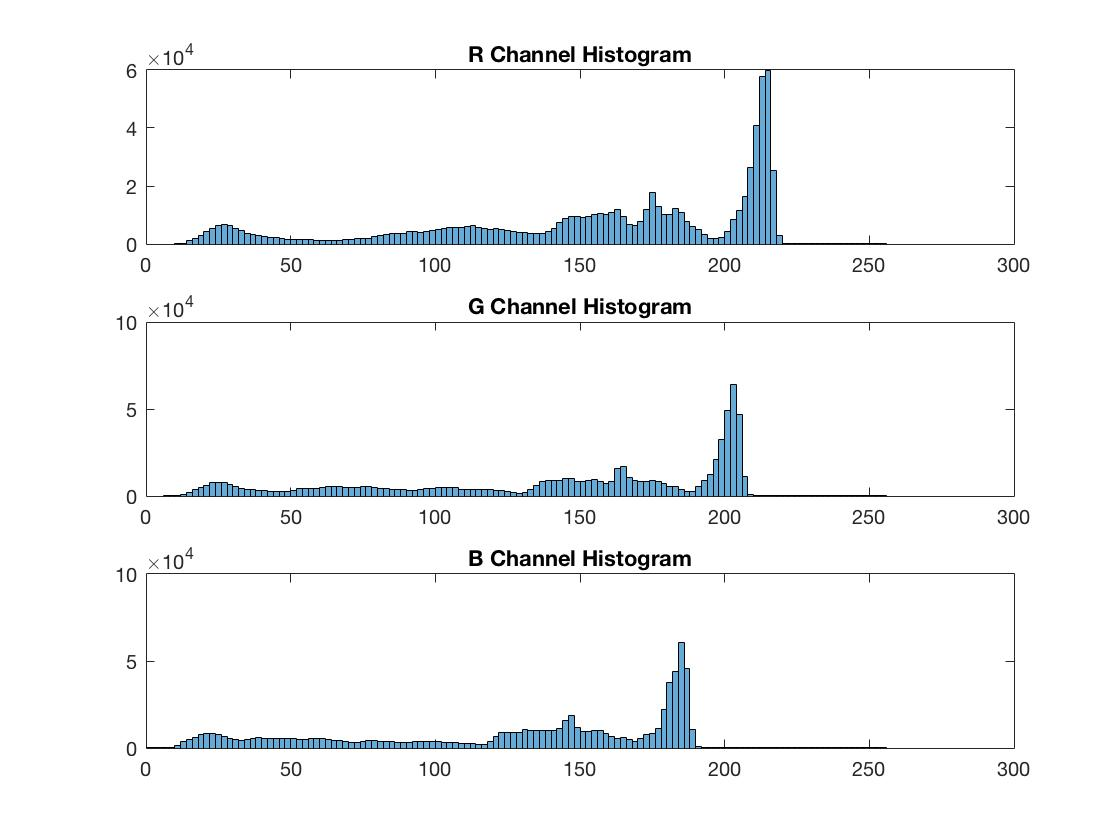
\includegraphics[scale = 0.3]{fig3.jpg}
    \caption{Histograms of RGB channels}
    \label{fig3}
\end{figure}

\subsubsection*{3.5 Apply the same methods to the resized picture}
The codes of this task is almost similar to the former ones. So I just show the results here. Remember that the resized picture has been shown before.
\begin{figure}[htbp]
    \centering
    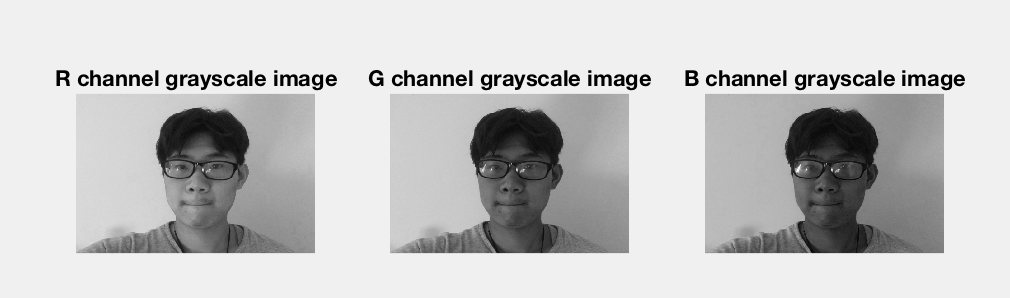
\includegraphics[scale = 0.6]{fig4.jpg}
    \caption{RGB gray scale images of resized picture}
    \label{fig4}
\end{figure}
\begin{figure}[htbp]
    \centering
    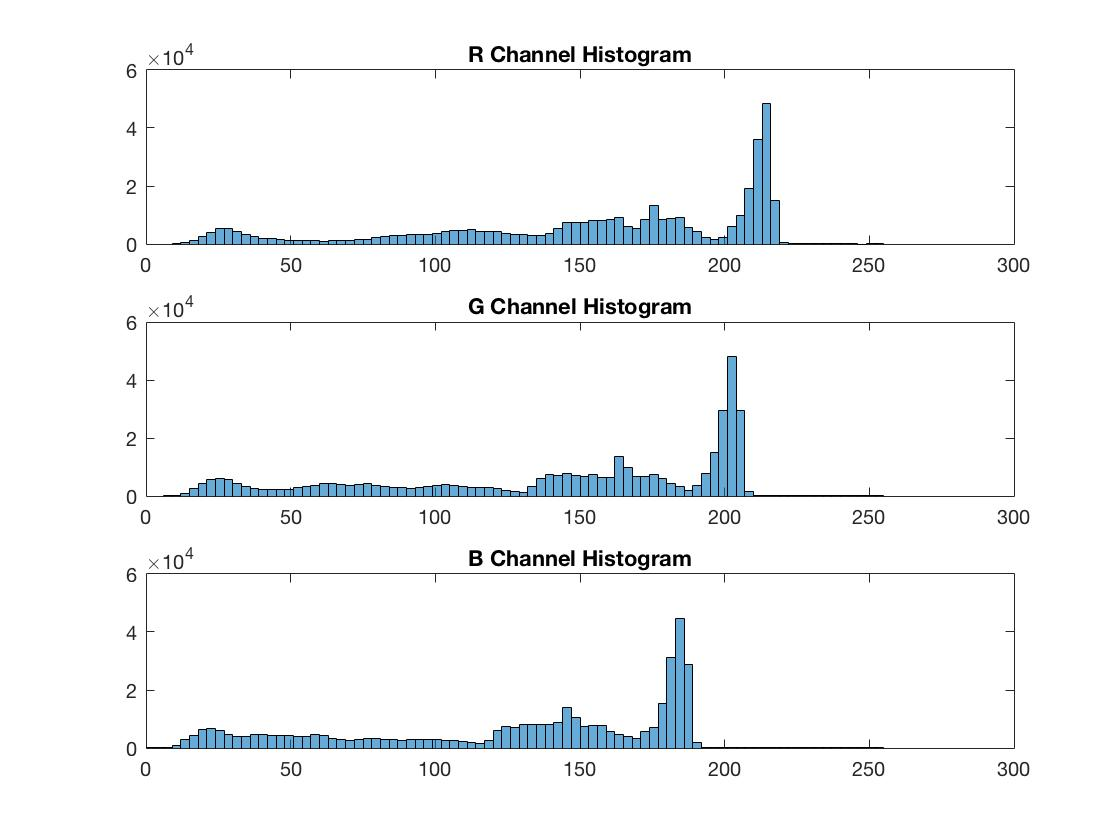
\includegraphics[scale = 0.3]{fig5.jpg}
    \caption{Histogram of resized RGB channels}
    \label{fig5}
\end{figure}



\section{Task 2: Colour Name Recognition}
\subsubsection*{Step 1 \& Step 2: Convert the picture to HSV picture and show the H image.}
These steps are easy to apply. I just use inbuilt matlab function $rgb2hsv()$ to get the result.
Codes:
\begin{lstlisting}
    input = 'colorwheel.jpg';
    origin = imread(input);
    edit = rgb2hsv(origin);
    figure;
    subplot(1,2,1);
    imshow(origin)
    title('origin iamge');
    subplot(1,2,2);
    imshow(edit(:,:,1));
    title('H Channel Image');
\end{lstlisting}

\begin{figure}[htbp]
    \centering
    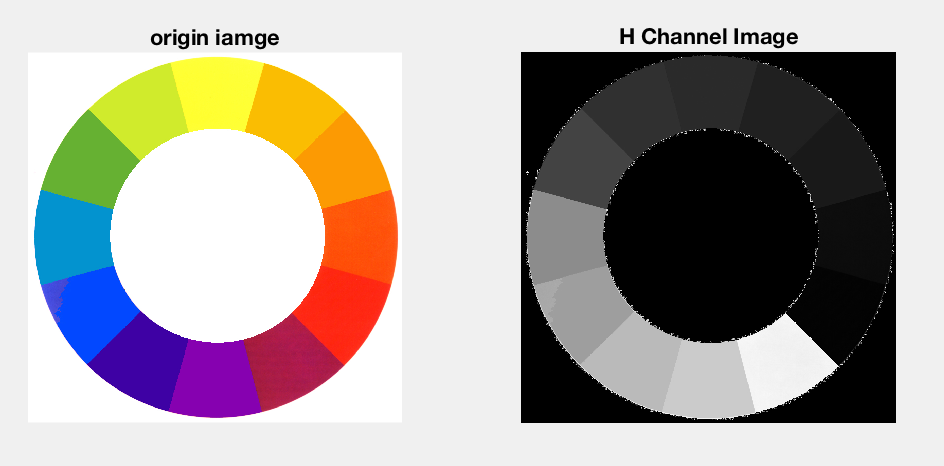
\includegraphics[scale = 0.6]{fig6.jpg}
    \caption{Convert RGB image to HSV image}
    \label{fig6}
\end{figure}

\subsubsection*{Step 3: Print the 12 average Hue-values next to the 12 colored regions in the image}
For this step, it is hard to use Matlab to auto detect the areas and calculate the values. So I detect the locations of each color first by using screen-shot tools. For each color, I choose a square which contains 400 pixels to represent the color. The selected areas are shown below.
\begin{figure}[htbp]
    \centering
    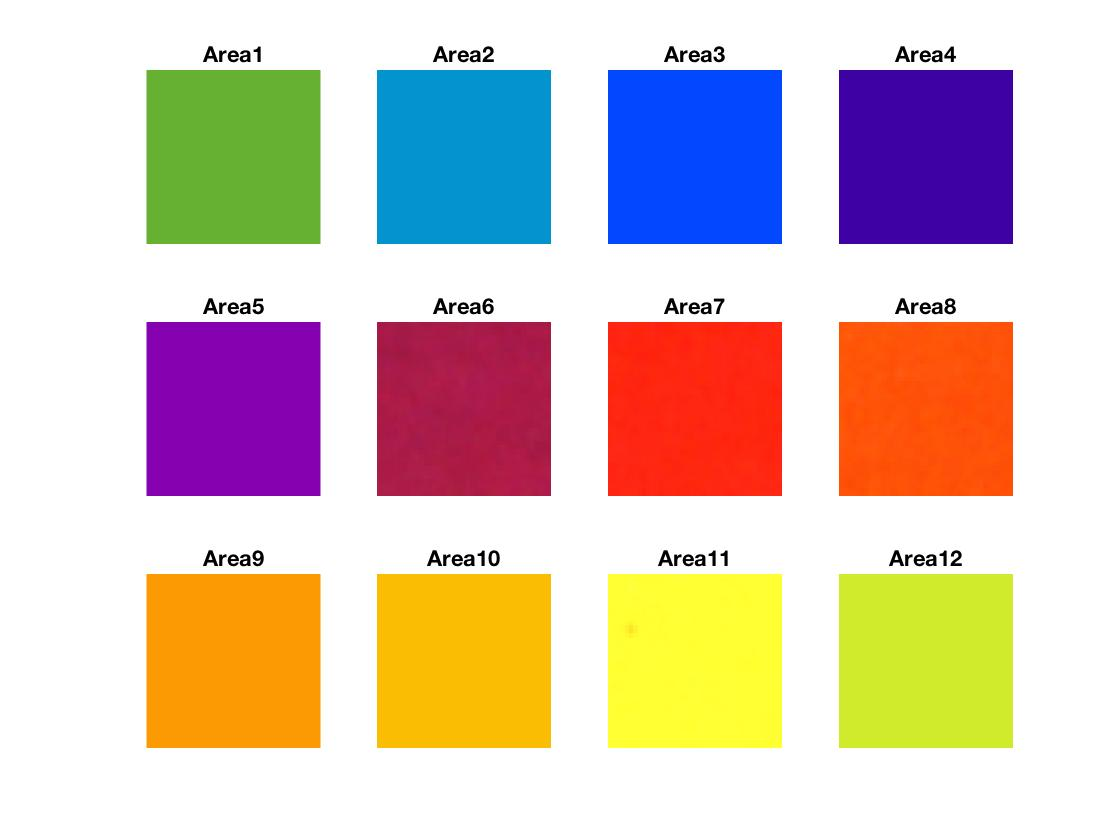
\includegraphics[scale = 0.2]{fig7.jpg}
    \caption{Selected areas for each color}
    \label{fig7}
\end{figure}

Then I print the H Value inside the area of that color in the H image. Here are the codes and the results.

Codes:
\begin{lstlisting}
    position_a = [340 534 738 906 968 934 750 548 326 182 140 194];
    position_b = [170 128 180 316 538 750 906 970 898 746 552 332];
    values = zeros(1,12);
    figure;
    for x = 1:12
        subplot(3,4,x);
        a = position_a(x);
        b = position_b(x);
        imshow(origin(a-20:a+20,b-20:b+20,:));
        values(x) = mean(mean(edit(a-20:a+20,b-20:b+20,1)));
        title(['Area' num2str(x)])
    end
    
    
    figure;
    imshow(edit(:,:,1));
    for y = 1:12
       content = ['Average Hue: ' num2str(values(y))];
       text(position_a(y),position_b(y),content ,'horiz','center','color','r');
    end

\end{lstlisting}

Result:
\begin{figure}[htbp]
    \centering
    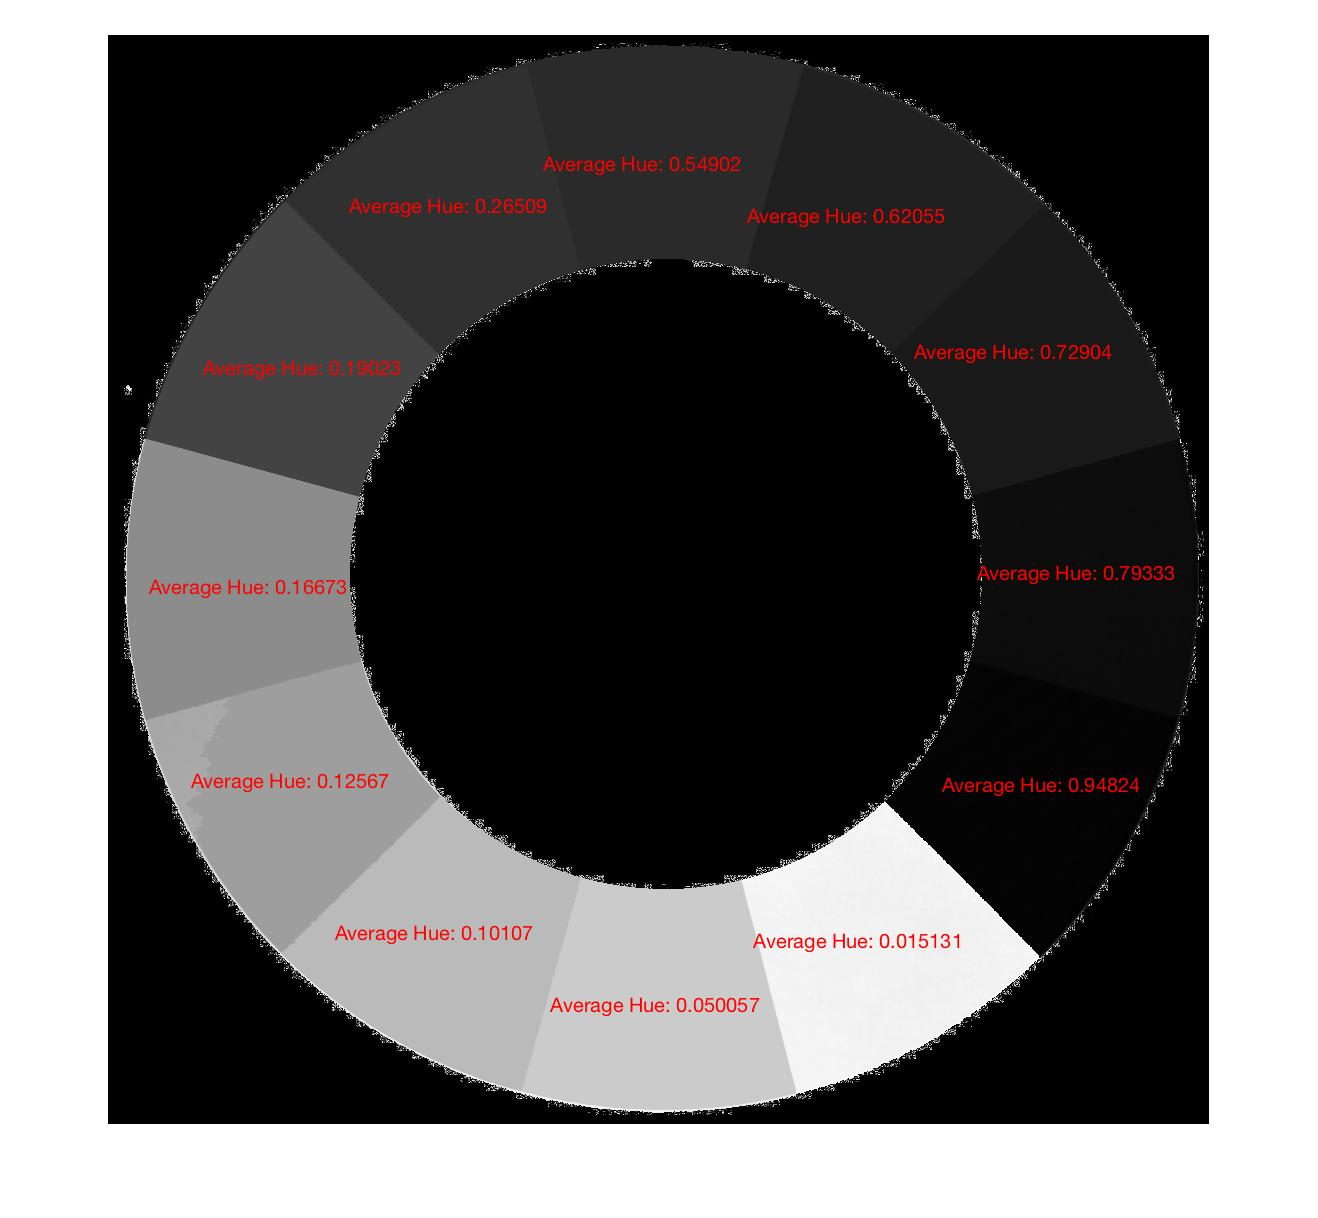
\includegraphics[scale = 0.15]{fig8.jpg}
    \caption{Result of Task 2}
    \label{fig8}
\end{figure}


\section{Task 3: Image denoise via Gaussian filter}
\subsection*{Step 1 \& Step 2: Read in one image and add Gaussian noise}
we can add Gaussian noise to an image easily by using Matlab inbuilt function $imnoise()$. The codes and the result of this Step are in the following.

Codes:
\begin{lstlisting}
    %step 1
    fin = imread('task3.jpg');
    edit = imresize(fin,[512 512]);
    edit_s = rgb2gray(edit);
    imwrite(edit_s,'3_1.jpg');
    %step 2
    noise_pic = imnoise(edit_s,'gaussian',0,30^2/255^2);
    noise_pic = double(noise_pic);
\end{lstlisting}

Result:
\begin{figure}[htbp]
    \centering
    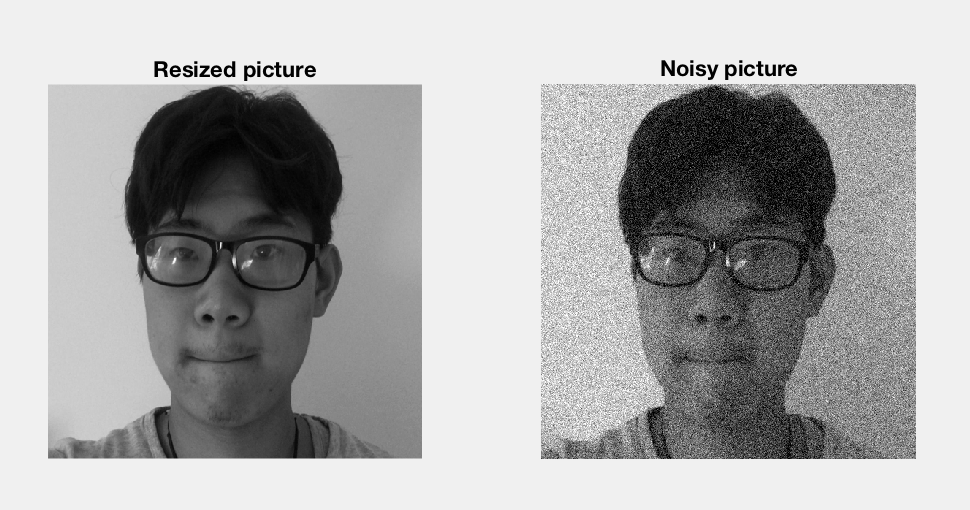
\includegraphics[scale = 0.6]{fig9.png}
    \caption{Resized and noisy pictures}
    \label{fig9}
\end{figure}

\subsection*{Step 3: Plot the two histograms side by side}

The codes of this step quite similar to task 1. I omit them here. Figure 10 shows the result of this step. 

\begin{figure}[htbp]
    \centering
    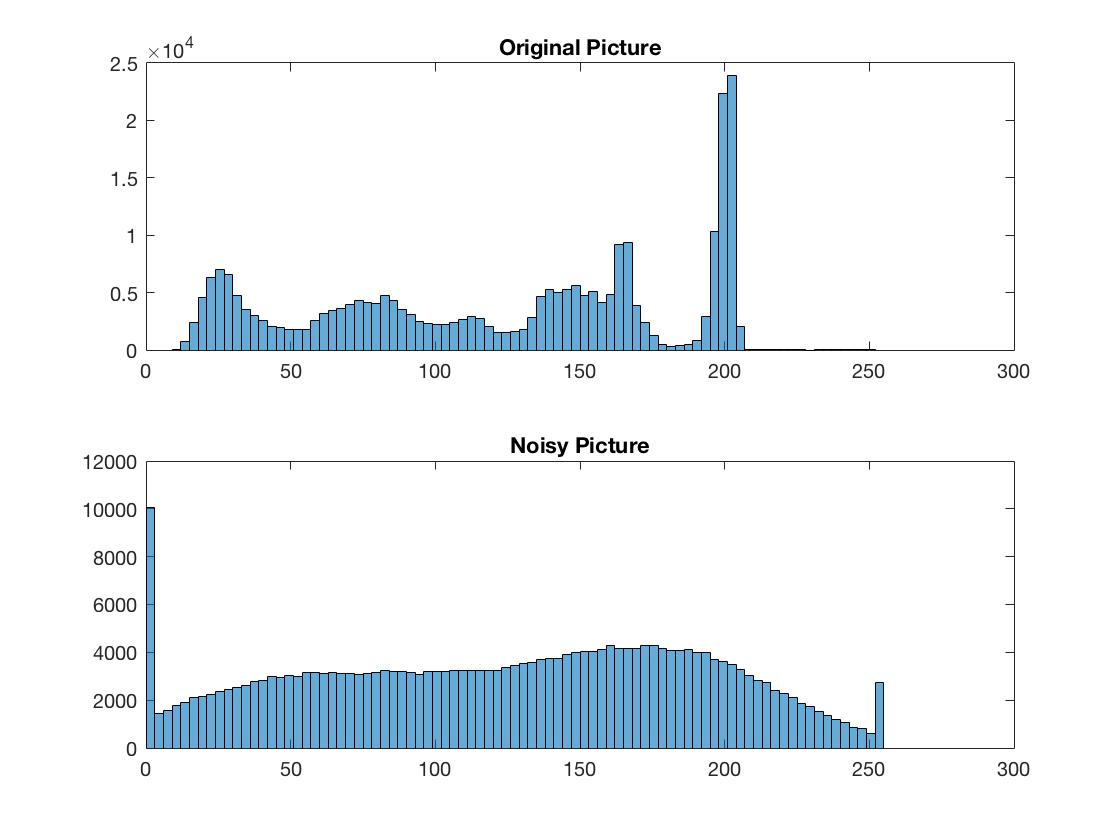
\includegraphics[scale = 0.3]{fig10.jpg}
    \caption{The histograms of the resized and noisy pictures}
    \label{fig10}
\end{figure}

\subsection*{Step 4 \& Step 5: Implement your own Gaussian function}

The actual question of this step is to implement one $filter$ or $conv2$ function as the Gaussian kernel is given. 

I write the following codes to finish this task. But one thing should be confirmed here: The processed image does not have the same size as the original image. I reduce 8 pixels, which are in the boundary of the image, in both width and length to finish the convolution. In my opinion, the size is not a initial problem. If we want to keep the same size as the original image, just keep the removed pixels the same as the original image. The codes for it is as simple as the following:

\begin{lstlisting}
    %im_out: ideal output
    %im_origin: original image
    %im_edit: output of my filter function
    im_out = im_origin;
    [a,b] = size(im_out);
    im_out(5:a-4,5:b-4) = im_edit;
\end{lstlisting}

The codes of this step:
\begin{lstlisting}
    %function codes:
    function im_out = my_Gauss_filter(noisy_image, my_9x9_gausskernel)
        %gauss_kernel should be prepared already
        [a,b] = size(noisy_image);
        im_out = zeros(a-8,b-8);
        gauss = reshape(my_9x9_gausskernel,[1,81]);
        
        for i = 1:a-8
            for j = 1:b-8
                img_window = noisy_image(i:i+8,j:j+8);
                img_window = reshape(img_window,[81,1]);
                im_out(i,j) = gauss*img_window;
            end
        end
    %main codes
    %step 4
    H = fspecial('gaussian',[9 9],30);
    denoise = my_Gauss_filter(noise_pic,H);
    figure;
    subplot(1,2,1)
    imshow(denoise,[]);
    title('my Gauss filter');
    %step 5
    denoise2 = filter2(H,noise_pic);
    subplot(1,2,2);
    imshow(denoise2,[]);
    title('Matlab Gauss Filter');
\end{lstlisting}

The result of my Gaussian filter and Matlab inbuilt Gaussian function are compared below (Gaussian kernel with SIGMA 30).

\begin{figure}[htbp]
    \centering
    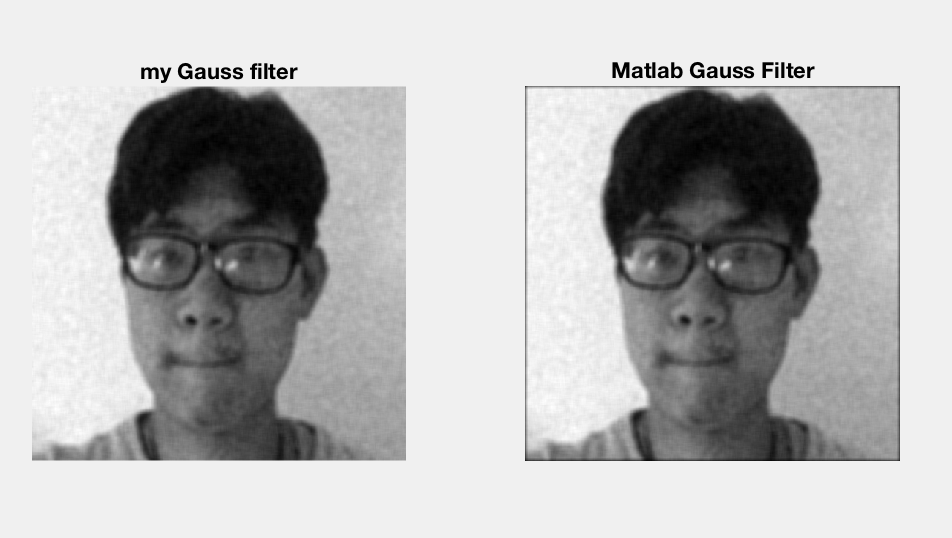
\includegraphics[scale = 0.6]{fig11.jpg}
    \caption{Result of my Gauss filter and Matlab inbuilt Gaussian filter}
    \label{fig11}
\end{figure}

The following 3 figures show the gaussian filter with SIGMA 1,10 and 50. We can see that a suitable SIGMA value can make sure the gaussian filter work well.

\begin{figure}[htbp]
    \centering
    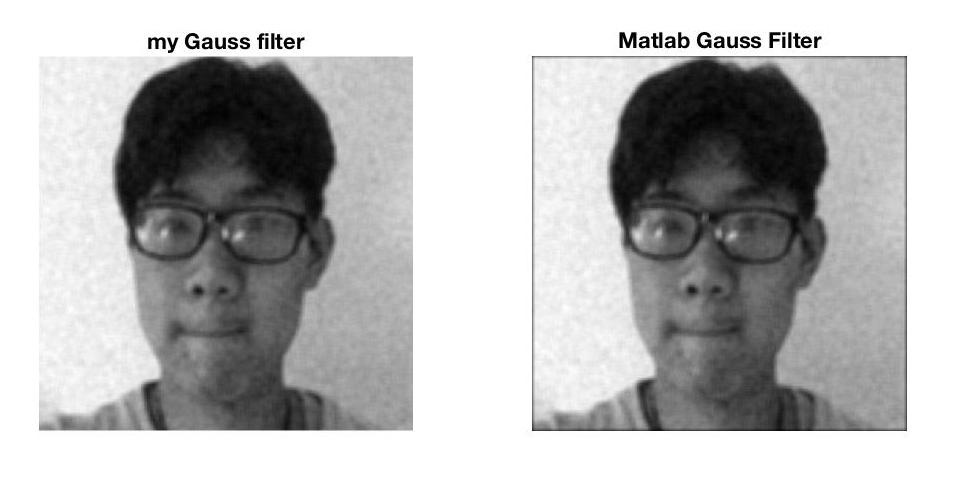
\includegraphics[scale = 0.3]{fig24.jpg}
    \caption{Result with Gasussian Filter (SIGMA 1)}
    \label{fig24}
\end{figure}
\begin{figure}[htbp]
    \centering
    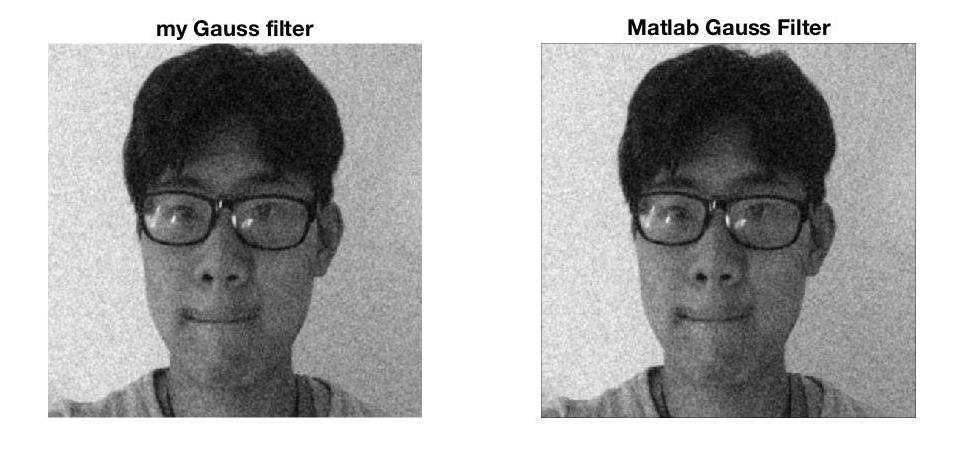
\includegraphics[scale = 0.3]{fig25.jpg}
    \caption{Result with Gasussian Filter (SIGMA 10)}
    \label{fig25}
\end{figure}
\begin{figure}[htbp]
    \centering
    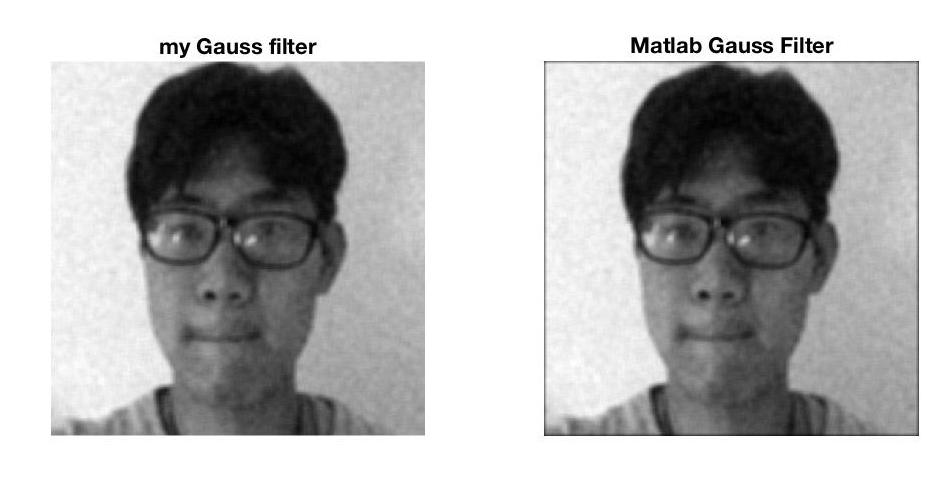
\includegraphics[scale = 0.3]{fig26.jpg}
    \caption{Result with Gasussian Filter (SIGMA 50)}
    \label{fig26}
\end{figure}

\section{Task 4: Implement your own $3\times3$ Median and Sobel Filter}
\subsection{Median Filter De-noise}
 
For this subsection, I first add 10\% salt and pepper noise to one of my original colour face image. It is needed to be explained that I change the color face to a gray scale face for further process as the de-noise process is quite the same for the three channels (RGB). The codes of this step are shown below. 
\begin{lstlisting}
    %step 1
    fin = imread('face_02_u6600985.jpg');
    fin = rgb2gray(fin);
    fin = double(fin);
    [a,b] = size(fin);
    tmp = reshape(fin,[a*b,1]);
    random_sequence = randperm(a*b);
    bound = floor(a*b/20);
    to1 = random_sequence(1:bound);
    to0 = random_sequence(bound+1:bound*2);
    tmp(to1) = 255;
    tmp(to0) = 0;
    tmp = reshape(tmp,[a b]);
    figure;
    imshow(tmp,[]);
\end{lstlisting}

Figure 15 shows the noisy picture.

\begin{figure}[htbp]
    \centering
    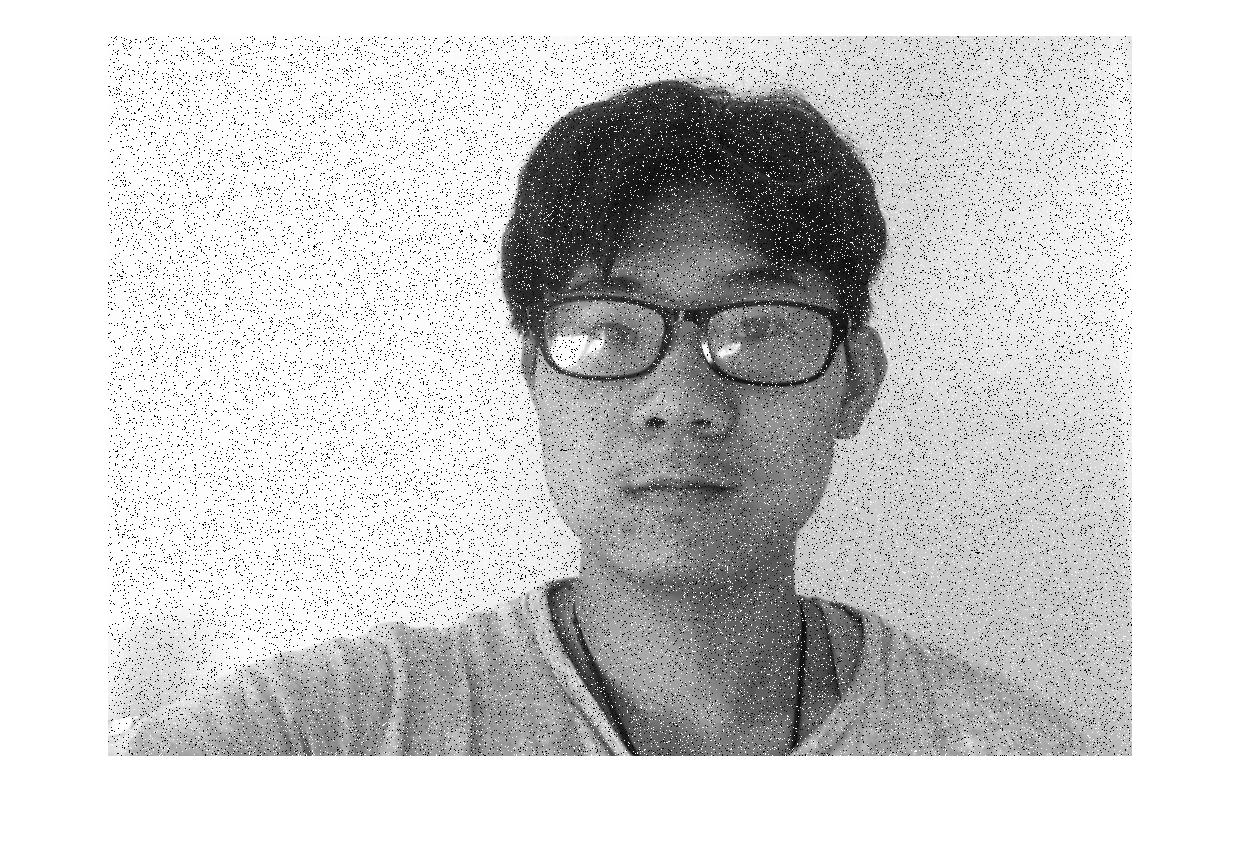
\includegraphics[scale = 0.25]{fig12.jpg}
    \caption{Picture with salt and pepper noise}
    \label{fig12}
\end{figure}

Then for the median filter, I wrote a function named $my\_median\_filter$ to finish the $3\times3$ median denoise. The codes of my function are as follows.

\begin{lstlisting}
    function im_out = my_median_filter(noisy_img)
    %this function denoise with a 3*3 median filter;
    [a,b] = size(noisy_img);
    im_out = zeros(a-2,b-2);
    
    for i = 1:a-2
        for j = 1:b-2
            img_window = noisy_img(i:i+2,j:j+2);
            img_window = sort(reshape(img_window, [9 1]));
            im_out(i,j) = img_window(5);
        end
    end
\end{lstlisting}

This function reduce 2 pixels in width and 2 pixels in length. But it can use the same method as gaussian function to keep the same size. Besides, this function also has one small problem comparing with Matlab inbuilt function. It takes a long time the finish the process as I wrote a loop with a sort. But for the inbuilt function, less time is cost. I think maybe the inbuilt function is written base on matrix methods and carries out an arithmetic optimization.

Figure 16 shows the deniose result in comparation with a inbuilt median filter.



\begin{figure}[htbp]
    \centering
    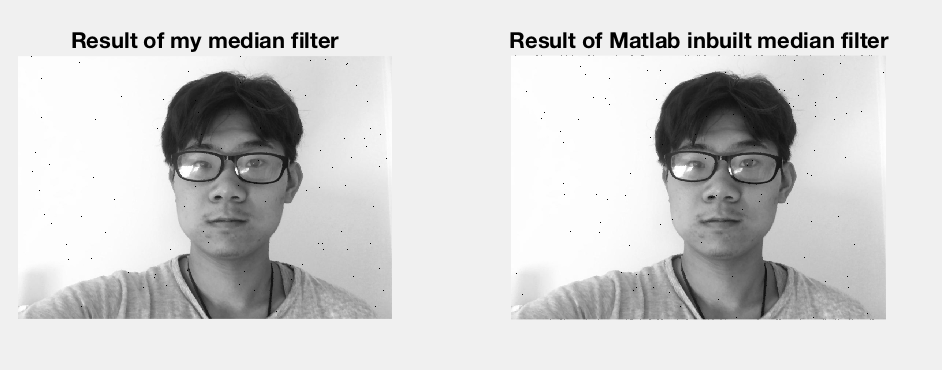
\includegraphics[scale = 0.6]{fig13.jpg}
    \caption{Result of my median filter and Matlab inbuilt median filter}
    \label{fig13}
\end{figure}

\subsubsection*{Q: Which filter (Gaussian or Median) is more suitable for removing salt-and-peper noise? Why?}
\textbf{A:}~~Figure 17 shows the result of Gaussian function and Median function of the same image. It is clear from the result that Median filter is more suitable for filtering SP noise and has a decent effect on it. The reason is that SP noise changes some pixels to totally black or white. The median filter is insensitive to extreme values but gaussian filter is.

\begin{figure}[htbp]
    \centering
    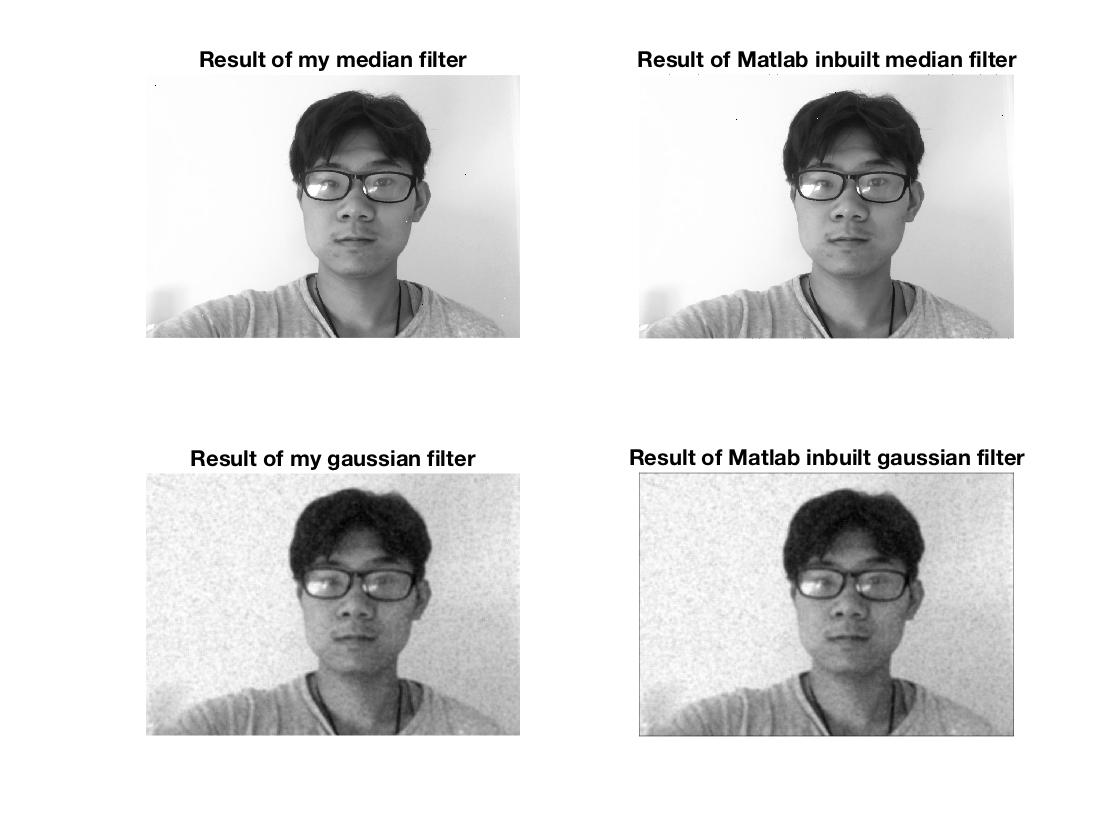
\includegraphics[scale = 0.25]{fig14.jpg}
    \caption{SP denoise with gaussian and median filters}
    \label{fig14}
\end{figure}

\subsection{Implement your own $3\times3$ Sobel edge detector}

For this task, I apply two kinds of sobel filters mentioned in the lecture. 

\begin{equation}
    \left(
    \begin{array}{ccc}
        1 & 0 & -1 \\
        2 & 0 & -2 \\
        1 & 0 & -1 \\
    \end{array}
    \right)
\end{equation}
and 
\begin{equation}
    \left(
    \begin{array}{ccc}
        1 & 2 & 1 \\
        0 & 0 & 0 \\
        -1 & -2 & -1 \\
    \end{array}
    \right)
\end{equation}

However, for Matlab inbuilt sobel filter, there is only one type. I compare the results of these three type of filters.

The codes of my sobel filters and the results of the three sobel filters are shown below.

\begin{lstlisting}
    function im_out = my_sobel_filter(img,mode)
    %this function denoise with a 3*3 sobel filter;
    filter1 = [1,0,-1,2,0,-2,1,0,-1];
    filter2 = [1,2,1,0,0,0,-1,-2,-1];
    if mode == 1
        myfilter = filter1;
    else
        myfilter = filter2;
    end
    [a,b] = size(img);
    im_out = zeros(a-2,b-2);
    
    for i = 1:a-2
        for j = 1:b-2
            img_window = img(i:i+2,j:j+2);
            img_window = reshape(img_window, [9 1]);
            im_out(i,j) = myfilter*img_window;
        end
    end
\end{lstlisting}

\begin{figure}[htbp]
    \centering
    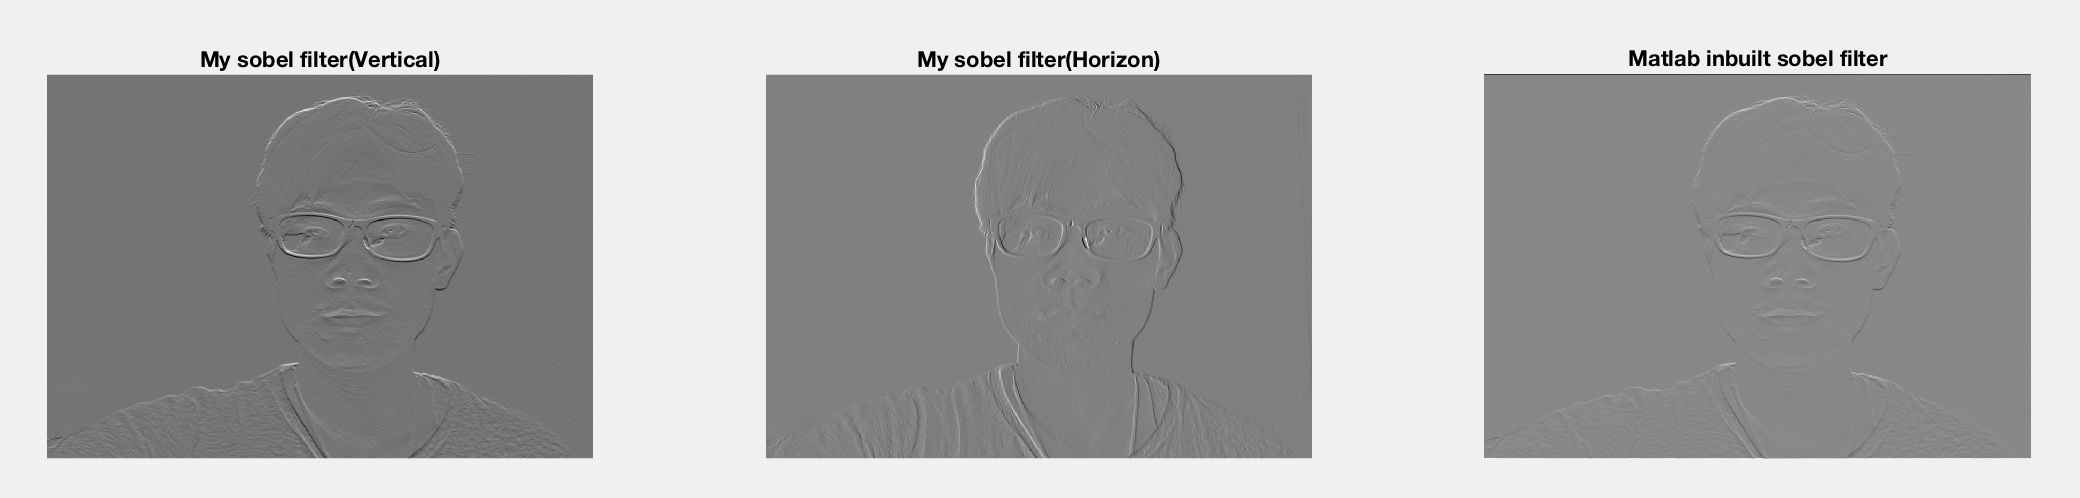
\includegraphics[scale = 0.3]{fig15.jpg}
    \caption{Results of three sobel filters}
    \label{fig15}
\end{figure}

From the results, we can see that the vertical sobel filters work almost the same as the Matlab inbuilt one. The small difference is because the inbuilt function make a further denoise to the processed image.

\section{Task 5: Image Morphology}
\subsection*{Step 1 \& Step 2: Convert the image to a gray scale image (then Binary image) and then count the black and white pixels}

For the second step, I choose the threshold 0.5. The codes of these steps are quite easy.

\begin{lstlisting}
    %step 1
    fin = imread('text.png');
    gray_image = rgb2gray(fin);
    gray_image = imresize(gray_image, [1024 1024]);
    figure;
    imshow(gray_image);
    title('Gray image of task 5')
    %step 2
    bw = im2bw(gray_image,0.5);
    black = length(find(bw == 0));
    white = length(find(bw == 1));
    whole = black + white;
    disp(['White Pixel: ' num2str(white) ', Black pixel: ' num2str(black) ', Whole pixel: ' num2str(whole)]);
\end{lstlisting}

Figure 19 shows the result of step 1.

\begin{figure}[htbp]
    \centering
    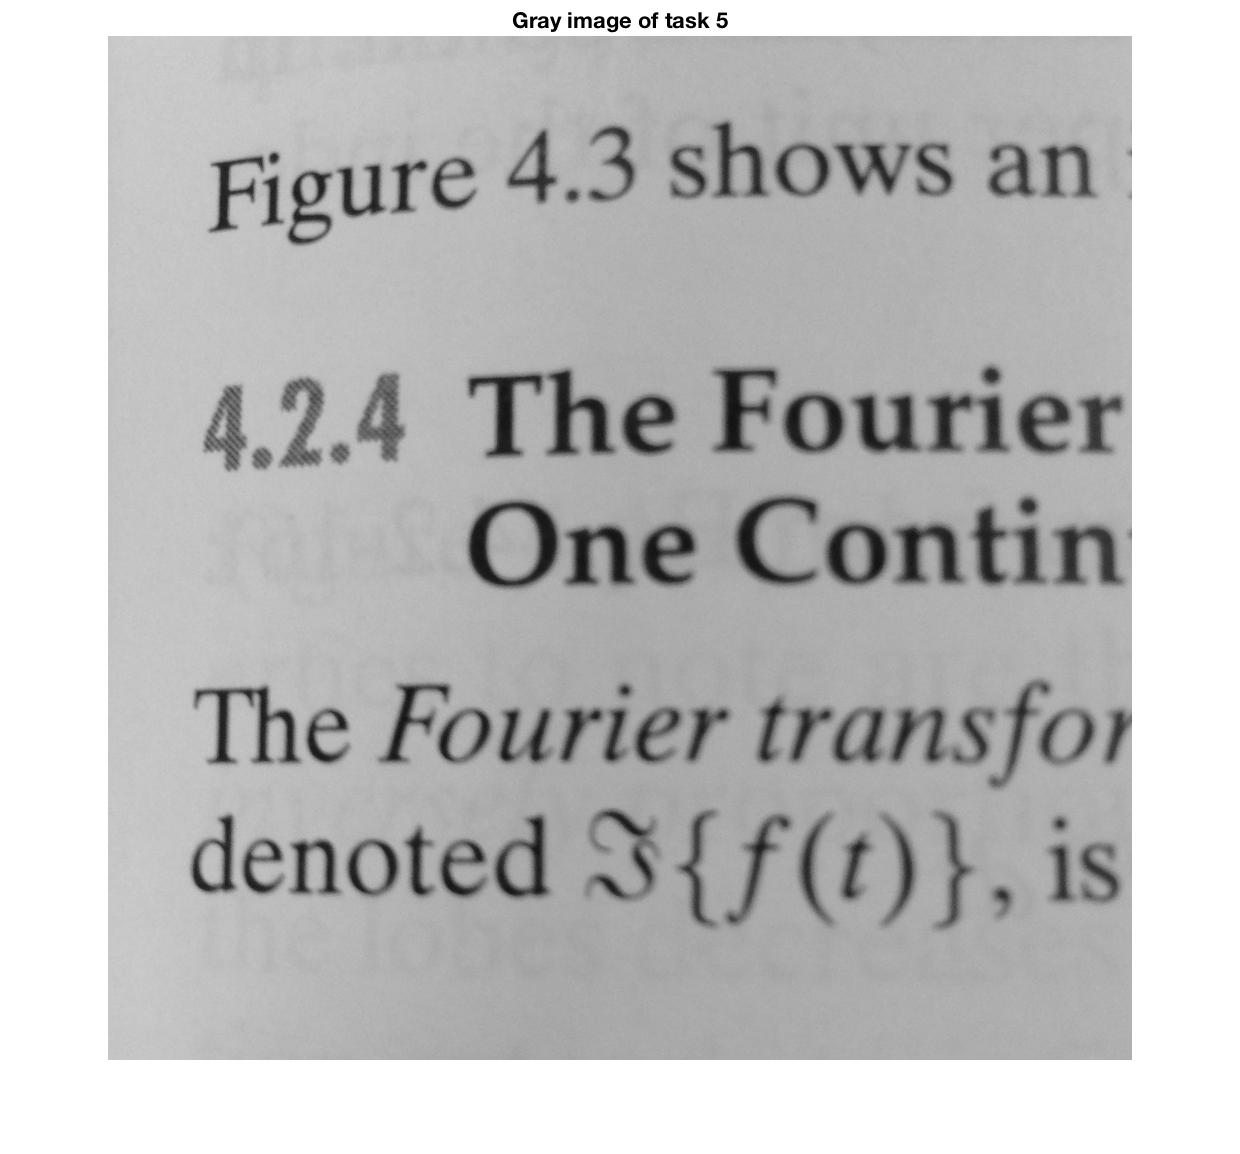
\includegraphics[scale = 0.15]{fig16.jpg}
    \caption{Converted and resized the picture}
    \label{fig16}
\end{figure}

Then the result of the couting process is:
$$White Pixel: 941192, Black pixel: 107384, Whole pixel: 1048576$$

\subsection*{Step 3: Testing the effects of applying Matlab inbuilt functions (``erosion", ``dilation", ``opening" and ``closing")}

I test these functions with different kernels which vary in size and form. The codes for these four functions are quite similar. I only put the codes of ``erosion" here. Just change the function ``imerode" to ``imdilate", ``imopen" and ``imclose" to get the other results.

Codes:
\begin{lstlisting}
    %step 3
    figure;
    %erosion
    ero_10 = zeros(1,10)+1;
    ero_101 = zeros(10,10)+1;
    erosion_img_h_10 = imerode(bw,ero_10);
    erosion_img_v_10 = imerode(bw,ero_10');
    erosion_img_s_10 = imerode(bw,ero_101);
    
    subplot(2,3,1)
    imshow(erosion_img_h_10);
    title('horizon erosion with index 10');
    subplot(2,3,2)
    imshow(erosion_img_v_10);
    title('vertical erosion with index 10');
    subplot(2,3,3)
    imshow(erosion_img_s_10);
    title('Square erosion with index 10');
    ero_30 = zeros(1,30)+1;
    ero_301 = zeros(30,30)+1;
    erosion_img_h_30 = imerode(bw,ero_30);
    erosion_img_v_30 = imerode(bw,ero_30');
    erosion_img_s_30 = imerode(bw,ero_301);
    
    subplot(2,3,4)
    imshow(erosion_img_h_30);
    title('horizon erosion with index 30');
    subplot(2,3,5)
    imshow(erosion_img_v_30);
    title('vertical erosion with index 30');
    subplot(2,3,6)
    imshow(erosion_img_s_30);
    title('Square erosion with index 30');
\end{lstlisting}

Figure 20 show the results of erosion. Function $imerode$ erases pixels horizontally or vertically or by square. It can be seen from the following image that with the increasing of vector (matrix) size, the erosion effect gets stronger. 

\begin{figure}[htbp]
    \centering
    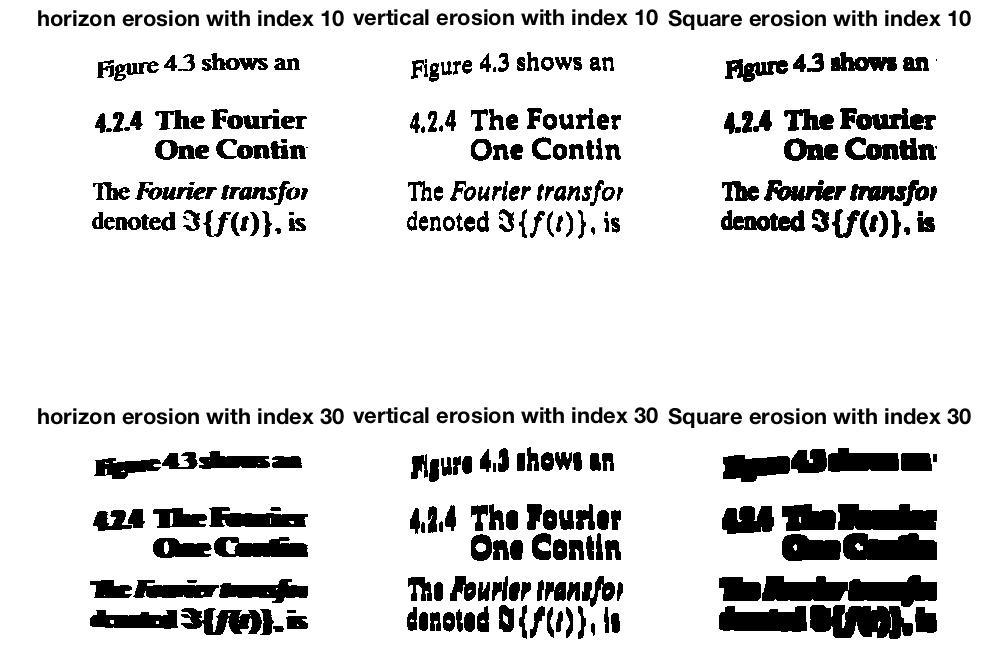
\includegraphics[scale = 0.28]{fig17.jpg}
    \caption{Results of image erosion}
    \label{fig17}
\end{figure}

Figure 21 show the results of dilation. Function $imdilate$ dilates pixels horizontally or vertically or by square. It can be seen from the following image that with the increasing of vector (matrix) size, the erosion effect gets stronger. 


\begin{figure}[htbp]
    \centering
    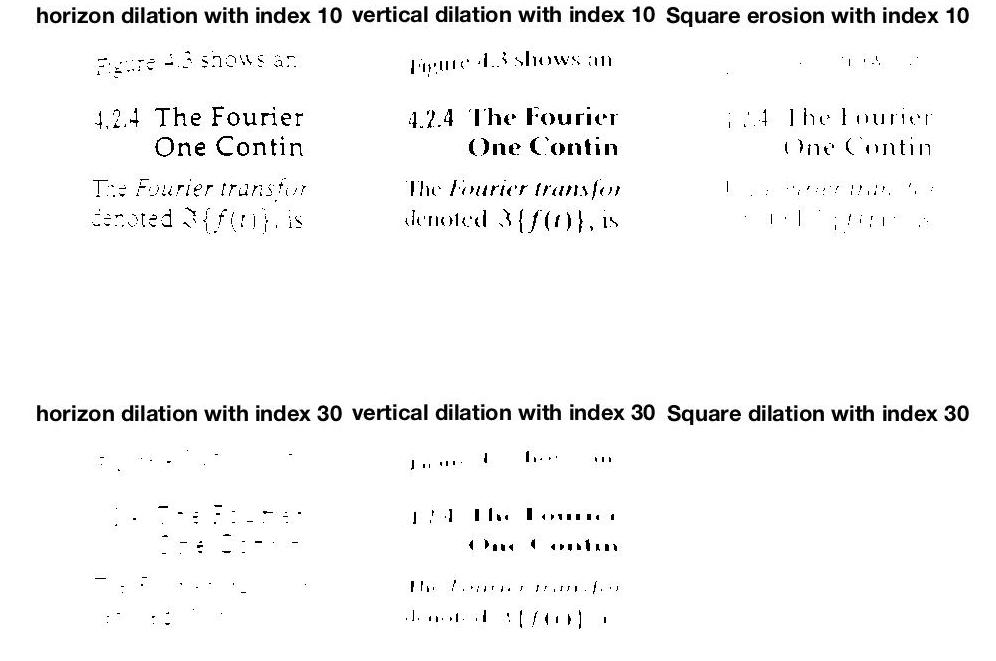
\includegraphics[scale = 0.28]{fig18.jpg}
    \caption{Results of image dilation}
    \label{fig18}
\end{figure}

Figure 22 show the results of opening. As introduced in the lecture, opening is an operation includes erosion and dilation. With dilation implemented after erosion, the effect of opening would be erasing pixels. Function $imopen$ does the process horizontally or vertically or by square. The results of image opening with different kernels are shown below. 

\begin{figure}[htbp]
    \centering
    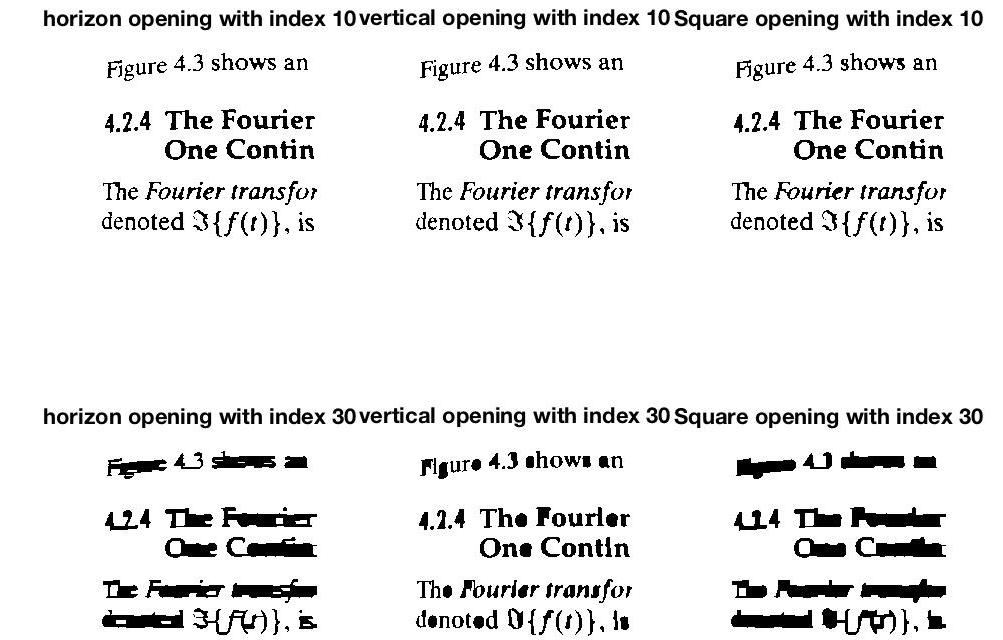
\includegraphics[scale = 0.28]{fig19.jpg}
    \caption{Results of image opening}
    \label{fig19}
\end{figure}

Similarly to opening, closing is an operation includes erosion and dilation. The only difference between closing and opening is the sequence of erosion and dilation. As a result, the effect of opening is equivalent to that of dilation. The results of horizontal, vertical and square closing with different size of vector can be seen as follow:

\begin{figure}[htbp]
    \centering
    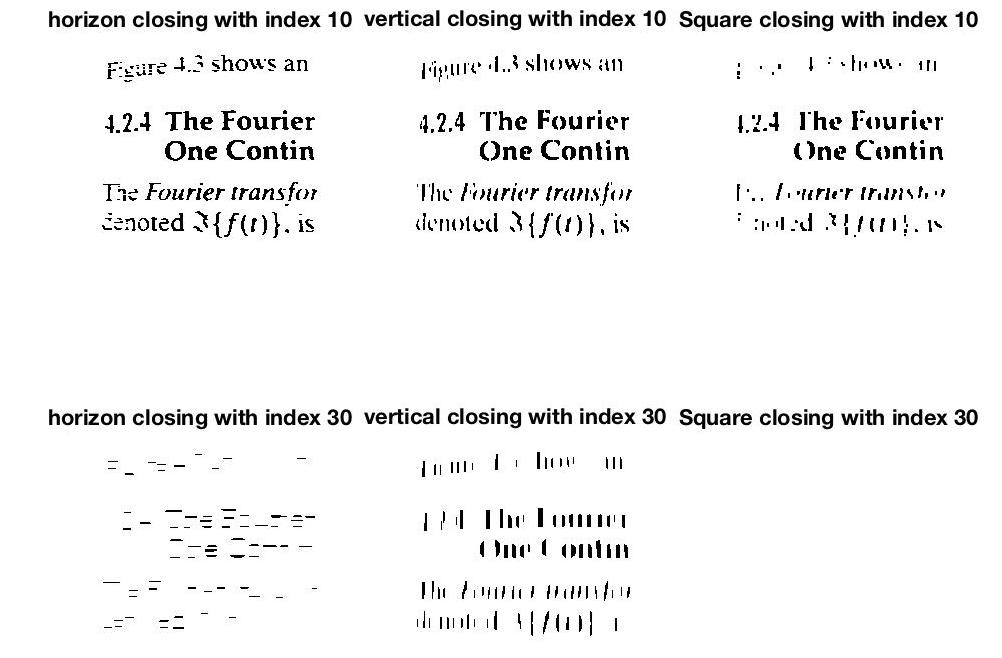
\includegraphics[scale = 0.28]{fig20.jpg}
    \caption{Results of image closing}
    \label{fig20}
\end{figure}

\section{Task 6: Geometric transformation}

For this task, I wrote two types of codes. At first, I follow the hint and write two rotate methods: forward rotate and inverse rotate. I test the forward method first. 

The codes and the results are shown as follow.

\begin{lstlisting}
    [h,w]=size(origin_img);  
    angle=angle/180*pi;
    c = cos(angle);  
    s = -sin(angle);  
    for i = 1:h
        for j = 1:w
            coor = [cos(angle), -sin(angle);sin(angle),cos(angle)]*[i;j];
            coor(1) = coor(1)+h;
            im_out(round(coor(1)),round(coor(2))) = origin_img(i,j);
        end
    end
\end{lstlisting}

\begin{figure}[htbp]
    \centering
    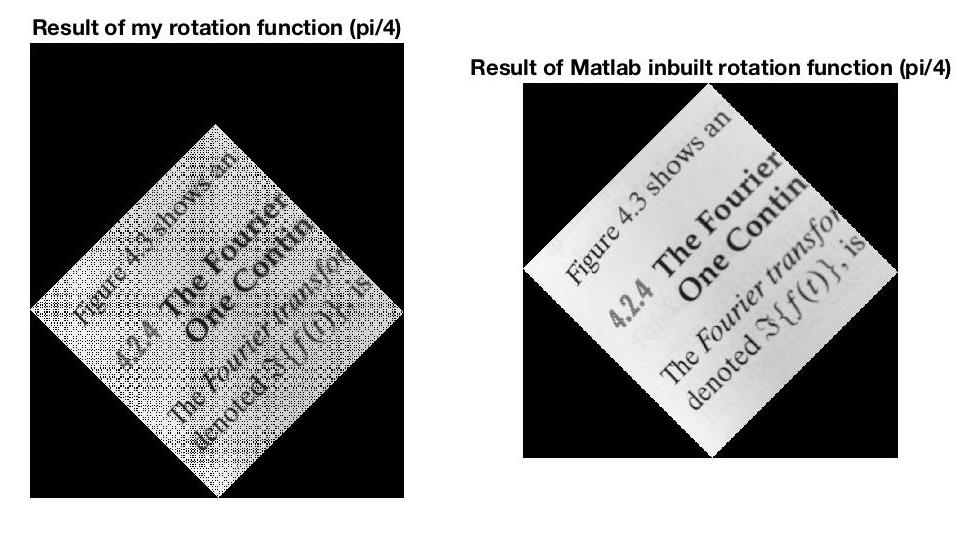
\includegraphics[scale = 0.25]{fig21.jpg}
    \caption{Rotate 45 angles with initial method}
    \label{fig21}
\end{figure}

\subsection*{Q: The differece between my function and Matlab inbuilt function}
\textbf{A: }~I found there are some fuzzy part in the picture processed by my filter. I think about the problem and found the reason. Not every pixel in the rotated picture has the corresponding pixel in the original image. Besides, two pixels may match the same pixel in the rotated image. So I change my mind and think about another method: Change the method and find the pixels from the original image which correspond to the rotated image. By applying this method, we can also avoid carrying out a classification discussion on angle.

Then I wrote the following codes based on some mathematical derivation and reference.
\begin{lstlisting}
    function im_out = rotate_img(origin_img,angle)
    [h,w]=size(origin_img);  
    angle=angle/180*pi;
    c = cos(angle);  
    s = -sin(angle);  
    
    w2=round(abs(c)*w+h*abs(s));  
    h2=round(abs(c)*h+w*abs(s));  
    im_out  = uint8(zeros(h2,w2));
      
      
    for x=1:w2  
        for y=1:h2  
            x0 = double(x*c + y*s -0.5*w2*c-0.5*h2*s+0.5*w);  
            y0= double(y*c-x*s+0.5*w2*s-0.5*h2*c+0.5*h);               
            x0=round(x0);          
            y0=round(y0);          
            if x0>0 && y0>0&& w >= x0 && h >= y0  
                im_out(y,x) = origin_img(y0,x0);  
            end  
        end  
    end  
\end{lstlisting}

Figure 25 and Figure 26 show the result of my rotation function and Matlab inbuilt function. This time, the two pictures keep the same. I think the inbuilt function is also based on the same algorithm.

\begin{figure}[htbp]
    \centering
    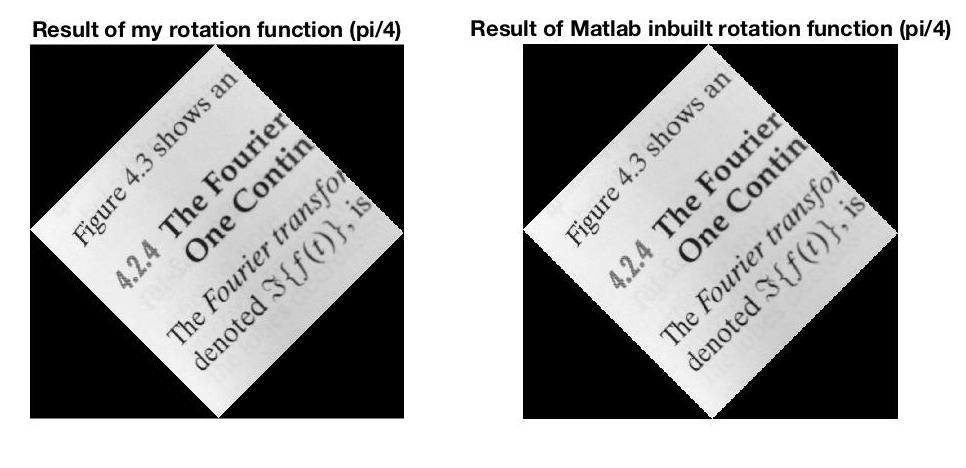
\includegraphics[scale = 0.25]{fig22.jpg}
    \caption{Rotate 45 angles with two types of methods}
    \label{fig22}
\end{figure}

\begin{figure}[htbp]
    \centering
    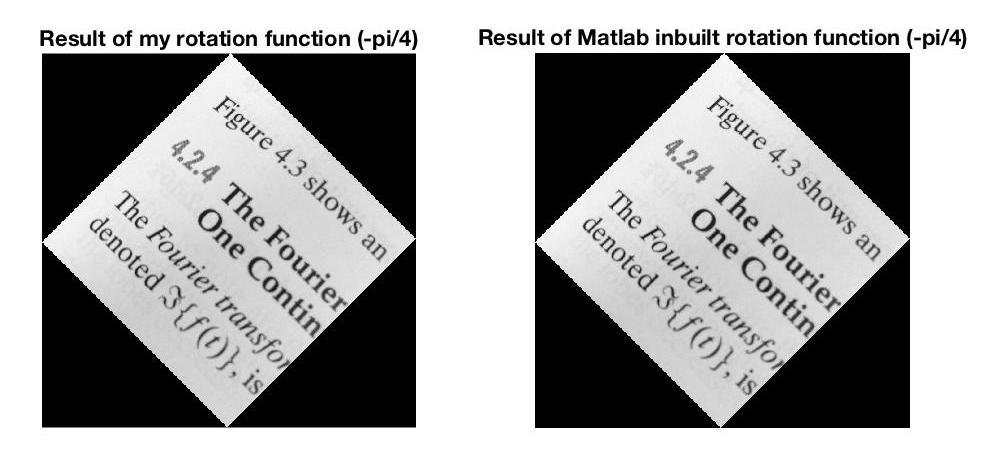
\includegraphics[scale = 0.25]{fig23.jpg}
    \caption{Rotate -45 angles with two types of methods}
    \label{fig23}
\end{figure}

\end{document}
